\begin{figure}[htp]
\centering
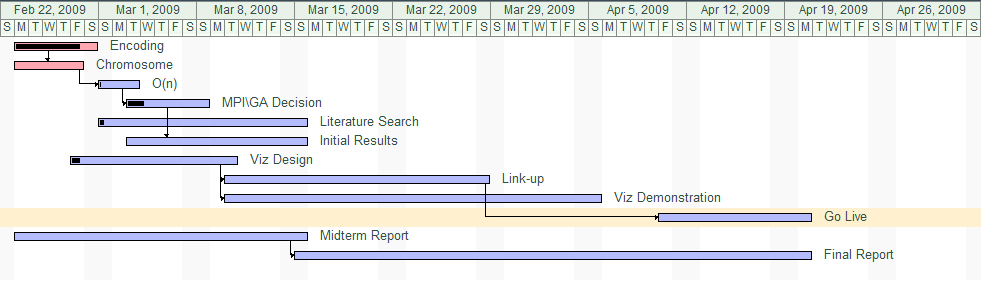
\includegraphics[width=1\textwidth]{images/gantt.png}
\caption{Project timeline of major milestones}\label{fig:gantt}
\end{figure}
Figure \ref{fig:gantt} shows a detailed timeline for the completion of the project. The major milestones for all aspects of the project present, including necessary work for the creation of an optimization scheme to search for UTMs as well as the creation of a web based visualization tool to facilitate the examination of the project results. The key to the task names used in Figure \ref{fig:gantt} is presented below: 
\begin{itemize}
	\item {\bf Encoding}:	Definition of the encoding method for TMs
	\item {\bf Chromosome}: Implementation of the chromosome class for the GA
	\item {\bf O(n)}:	Computational cost for fitness evaluation of a TM is determined.
	\item {\bf MPI/GA Decision}:	Decision made regarding necessity of use for MPI along with Genetic Algorithm to reduce computation time.
	\item {\bf Literature Search}: Literature search to generate a list of known UTMs
	\item {\bf Initial Results}: Initial TM optimization run completed. Data analyzed to ensure the viability of optimization scheme
	\item {\bf Viz Design}: Visualization web-app design complete
	\item {\bf Link-up}: Link between GA generation data and visualization database completed.
	\item {\bf Viz Demonstration}: Ruby on Rails visualization application implementation completed.
\end{itemize}
